\documentclass[11pt]{article}

\usepackage[margin=1in]{geometry}
\usepackage{amsmath, amssymb, amsthm}
\usepackage{booktabs}
\usepackage{tabularx}
\usepackage{array}
\usepackage{enumitem}
\usepackage{microtype}
\usepackage[hidelinks]{hyperref}
\usepackage[numbers,sort&compress]{natbib}
\usepackage{xcolor}
\usepackage{graphicx}

\newcolumntype{L}{>{\raggedright\arraybackslash}X}

\theoremstyle{plain}
\newtheorem{proposition}{Proposition}
\newtheorem{theorem}{Theorem}
\newtheorem{corollary}{Corollary}
\theoremstyle{definition}
\newtheorem{assumption}{Assumption}
\newtheorem{observation}{Observation}
\theoremstyle{remark}
\newtheorem{remark}{Remark}

\newcommand{\Jrt}{J_{\mathrm{rt}}}
\newcommand{\Jml}{J_{\mathrm{ml}}}
\newcommand{\kgraph}{\kappa_{\mathrm{graph}}}
\newcommand{\kgf}{\kappa_{\mathrm{gf}}}

\title{The Infeasibility of Mastery-Gated Curriculum Learning\\
for Language Model Pretraining}
\author{P4 Hypothesis Project}
\date{Working Draft, August 2026}

\begin{document}

\maketitle

\begin{abstract}
Mastery-gated curriculum learning organizes training content into a prerequisite
graph and unlocks a node only once its parents have been certified as mastered by
held-out probes. We argue that this design is structurally infeasible for
language model pretraining, and we do so without relying on the idealized
learning model that a companion formalization assumes. Our argument
has six parts, each priced with concrete numbers. First, a skill that has been
mastered does not stay mastered. In our own five-seed experiments the pure gating
policy (the one an idealized exposure model certifies as optimal) loses
$62.3\%$ of peak accuracy, against $1.3\%$ for a shuffled baseline. Second,
certification is expensive. Gate probes consume $11.8\%$ of training FLOPs in our
harness and, extrapolated to a $10^4$-node curriculum at OLMo-7B scale, between
$8.3\%$ and $125\%$ of the training budget, or \$0.42M--\$6.37M at Llama-3 scale.
Third, and decisively, certification is unreliable at any price. Because
checkpoint-to-checkpoint noise does not shrink with the probe budget, the
per-gate error rate converges to a positive constant, so gate cost is unbounded
above while gate reliability is bounded below. We measure that noise directly on
our own gate probes and find the mastery bit flips on $5.7\%$ of adjacent
checkpoint pairs, with $37.9\%$ of skills that once cleared the threshold later
falling back below it \emph{while still being trained on}. Fourth, the graph is
quadratic to build and cannot be accurate. Human annotators agree with their own
consensus at only $0.75$ F1, and at the true $2\%$ base rate of prerequisite
relations the implied precision is near $0.10$. Fifth, separating the two things
a gated curriculum does, we find that the prerequisite \emph{ordering} carries
the entire benefit (clock-staged training through a correct order beats no
graph by $+0.344$), while the \emph{gate} is negative at every level of graph
correctness, in three of three conditions. Sixth, a static graph is dominated by
online selection that reads the model's current state at under $0.4\%$ overhead.
We are explicit about what would falsify each claim, and about where our own
evidence is weak. Our experiments are small, synthetic, and closer in structure
to post-training than to pretraining.
\end{abstract}

\section{Introduction}

A mastery-gated curriculum is defined by two commitments. Content is organized
into a prerequisite directed acyclic graph, and a node becomes available for
training only after its parents have been \emph{certified}, shown by evaluation
on held-out probes to clear a threshold $\tau$. The design is borrowed from
human education, where it is among the better-attested interventions, and it has
an obvious appeal for pretraining. If a model must learn arithmetic before
algebra, why spend gradient steps on algebra first?

A companion document formalizes a bound on what the graph can contribute and
proves, in a machine-checked exposure model, that the marginal speedup of the
graph over a strong graph-free scheduler is capped by $c_x/f$, where $f$ is the
fraction of cost spent on incompressible content and $c_x$ prices the one channel
by which skill ordering could cheapen fact acquisition. That result is correct
within its model. Its model is also its weakness. Mastery of an item is defined
as
\[
\mathrm{mastered}(m,\sigma,i) \;:=\; m_i \le \mathrm{exposures}(\sigma, i),
\]
which is monotone in an item's own exposure count and wholly independent of every
other item. Both properties are false of real training, and a reader is entitled
to discount a conclusion that rests on them.

This paper makes the case again without that model. We replace the idealized
premises with measured quantities, and we find that the conclusion strengthens
rather than weakens. Every empirical correction to the exposure model adds cost
to the gated arm, and one of them, the irreducible noise floor of checkpoint
evaluation, converts a cost argument into an impossibility argument.

\paragraph{Structure of the argument.} Table~\ref{tab:roadmap} lists the seven
claims and, for each, the observation that would defeat it.
Section~\ref{sec:threats} then states the strongest objections we know of,
including the places where our own evidence is weak and one scale trend in the
literature that runs against us.

\paragraph{What we do not claim.} We do not claim that data ordering is
irrelevant, that curricula never help, or that scheduling research is
misdirected. Several of the results we rely on show the opposite in narrow
regimes. Our claim is specific. The \emph{gating} construct, a pre-committed
prerequisite graph whose edges are released by threshold-crossing
certification, is dominated on every axis we can measure, and what dominates it
is the absence of a curriculum.

\paragraph{Who holds the position we are arguing against.} No published system
implements mastery gating for language model pretraining, and we should say so
plainly rather than imply we are refuting an established practice. What exists is
a widely held intuition, an adjacent literature that formalizes curricula as
prerequisite DAGs with threshold-gated advancement in reinforcement learning
\citep{narvekar2020curriculum,svetlik2017automatic}, production systems that gate
on success thresholds \citep{akkaya2019solving,openended2021xland}, and a
companion formalization of our own that appears to license the design. A
proof-style paper is the right instrument precisely because the position is
prospective. The argument is that the design should not be built, and the
evidence is what it would cost and whether its central measurement is
obtainable.

\paragraph{What regime our experiments occupy.} Our runs are pretraining in
mechanics and post-training in structure, and it is better to say so than to let
a reader discover it. They start from random initialization and train for
$6{,}000$ steps with no pretrained base, which is pretraining. But the data are
procedurally generated task instances with exact-match answers, evaluation is a
frozen per-skill probe set, and the loss is masked to answer tokens with prompt
positions ignored, which is the supervised fine-tuning convention, not the
language-modelling one. The most accurate description is from-scratch supervised
fine-tuning on synthetic tasks.

This matters for which claims our experiments can support. The reliability floor
of Section~\ref{sec:reliability} is indifferent to the training objective. It
needs only a noisy measurement compared against a threshold. So are the decay and
gating results, which concern the advancement rule rather than the loss. The
arguments that genuinely require pretraining scale (the $10^{10}$-node graph
cost, the dollar figures, the reasoning about a fact-dominated corpus) rest on
the literature, and our runs neither corroborate nor contradict them. Readers who
think mastery gating is really a post-training proposal should note that the
cost arguments weaken in that setting, since a post-training curriculum has
hundreds of skills rather than billions of documents, while the reliability and
staleness arguments survive intact and arguably strengthen, because gates
certified by sampled rollouts are noisier than gates certified by scoring.

\begin{table}[ht]
\centering
\small
\begin{tabularx}{\textwidth}{@{}c L L@{}}
\toprule
\S & Claim & Would be falsified by \\
\midrule
\ref{sec:decay} & Mastered skills decay, so gates must recur &
  Competence shown stable across checkpoints without re-exposure \\
\ref{sec:probecost} & Certification is expensive &
  Nothing; this is token accounting, not an empirical claim \\
\ref{sec:reliability} & Certification is unreliable at \emph{any} budget &
  $\sigma_{\text{ckpt}} \approx 0$ at pretraining scale (we measure $0.023$ on
  our own gate probes) \\
\ref{sec:graphcost} & The graph is quadratic to build and cannot be accurate &
  An extractor exceeding $0.75$ F1 against an independent gold standard \\
\ref{sec:wrong} & The ordering carries the benefit; the gate subtracts &
  A gated arm beating a clock on the same graph, at any graph quality \\
\ref{sec:static} & Given structure, reading model state beats pre-committing &
  A pre-committed schedule beating online reweighting on the same structure \\
\ref{sec:human} & The human mechanism has no analog &
  A knowledge-dependent capacity limit in transformers \\
\bottomrule
\end{tabularx}
\caption{The argument at a glance, with the observation that would defeat each
part. Sections~\ref{sec:probecost} and \ref{sec:reliability} carry the most
weight and depend on the fewest contested premises.}
\label{tab:roadmap}
\end{table}

\section{Mastery Decays}
\label{sec:decay}

\subsection{What the idealized model assumes}

The exposure model makes three assumptions, each of which is required for a gate
to be meaningful:

\begin{enumerate}[leftmargin=1.6em,itemsep=1pt]
  \item \textbf{Monotonicity.} Competence on item $i$ is nondecreasing in the
        exposures $i$ has received. Once mastered, always mastered.
  \item \textbf{Independence.} Competence on $i$ depends only on $i$'s own
        exposures, not on what else was trained.
  \item \textbf{Observability.} There is a measurement whose threshold crossing
        identifies the transition.
\end{enumerate}

Under these, the optimal schedule is immediate. Present each item exactly $m_i$
times and stop. Any exposure past threshold is waste. This is precisely what a
mastery gate implements, and it is why the idealized model endorses gating.

\subsection{Monotonicity fails, and the cost is large}

Table~\ref{tab:forget} reports peak-minus-final sealed accuracy across our
experimental arms, aggregated over all logged runs.\footnote{Reproduced by
\texttt{lean\_bound/analysis/forgetting\_audit.py}. Forgetting is the
Chaudhry-style measure, peak sealed accuracy over the run minus final, averaged
over skills.}

\begin{table}[ht]
\centering
\small
\begin{tabular}{@{}lrrrr@{}}
\toprule
Arm & Mean forgetting & Worst skill & Final acc. & $n$ \\
\midrule
\texttt{mastery\_naive} (gate, no replay) & \textbf{0.623} & \textbf{0.949} & 0.277 & 5 \\
\texttt{mastery\_replay} (gate $+$ $p{=}0.5$) & 0.019 & 0.143 & 0.792 & 5 \\
\texttt{fixed\_replay} (clock) & 0.023 & 0.260 & 0.835 & 5 \\
\texttt{shuffle} & 0.013 & 0.047 & 0.491 & 5 \\
\bottomrule
\end{tabular}
\caption{Retention loss by arm (E1, five seeds). The pure gating policy, which
stops sampling an item once it clears $\tau$, loses $62.3\%$ of peak accuracy on
average and $94.9\%$ on its worst skill. An independent replication (E3) gives
$0.685$ mean forgetting at replay fraction $p=0$.}
\label{tab:forget}
\end{table}

\begin{observation}[The certified-optimal policy is the worst arm]
\label{obs:worst}
The schedule that the exposure model proves optimal, presenting each item to
threshold and then stopping, is, in our runs, the worst-performing arm by final
accuracy, losing to undifferentiated shuffling by $0.214$ absolute.
\end{observation}

This is not an artifact of scale. The pretraining dynamics literature reports the
same phenomenon with a fitted functional form. \citet{chang2024acquire} inject
facts into OLMo checkpoints and resume real pretraining, finding that each
encounter produces an immediate rise in log-probability followed by decay that is
linear in $\log t$ with $R^2 > 0.80$ and a decay constant near $0.25$ for
OLMo-7B. Factual knowledge is the running sum of decaying impulses.
\citet{jagielski2023forgetting} identify the mechanism as
optimizer nondeterminism and show that \emph{deterministically} trained models do
not forget, which means decay is structural rather than incidental.
\citet{ibrahim2024simple} re-warm the learning rate while continuing
to train on the \emph{identical} distribution and still measure a $0.1$-nat
degradation. Competence erodes even when no new content is introduced.

\citet{chang2024acquire} also supply the construct that most cleanly replaces the
exposure counter. If a fact's inter-exposure interval exceeds a threshold, the
fact becomes unlearnable ``regardless of the duration of the pretraining.'' A
curriculum that certifies a unit and moves on drives that interval toward
infinity by design.

\subsection{Independence fails, sometimes catastrophically}

Interference is a first-order effect. The cleanest demonstration is in
pretraining itself. \citet{allenzhu2025capacity} show that when $7/8$ of training
tokens come from junk that is \emph{statistically independent} of the target
facts, capacity for the useful facts degrades by $20\times$ at 100 exposures,
recovering to $1.3\times$ only after $10\times$ more exposures. Nothing about the
junk relates to the targets, so this is interference rather than competition for
relevant signal. \citet{hernandez2022repeated} find that repeating $0.1\%$ of a
corpus roughly $100\times$ degrades an 800M model to the performance of a 340M
one, and does disproportionate damage to induction heads. Items compete for
shared circuits, not just storage.

The most dramatic figure in this literature needs a caveat we will supply
ourselves. \citet{lu2024factmemorization} train two fact types sequentially and
report that the earlier type's memorization rate falls from $20.9\%$ to zero,
symmetrically under reversal. That is a 41M--0.5B model trained from scratch on
tabular company facts in strictly sequential blocks, which is about the most
favourable possible setting for overwriting; we read the zero as an upper bound
on interference rather than a representative value. The direction is what the
argument uses, and the direction is corroborated by the two results above.

\citet{zucchet2025facts} localize the mechanism, in a fine-tuning setting rather
than a pretraining one. The collapse reproduces in an attention-free
single-hidden-layer associative memory, and attention patterns stay stable
throughout, so the corruption is in the feed-forward key--value store rather than
in attention drift.

The consequence for a gate is that $m_i$ is not a property of item $i$. It is a
property of item $i$ \emph{given the rest of the mixture}, and the mixture is
exactly what a curriculum changes.

\subsection{Observability fails because mastery is a relation, not a property}

Even granting a stable, independent competence, a gate needs to measure it.
\citet{allenzhu2024storage} exhibit a model with $99{+}\%$ first-token accuracy on
a fact and \emph{zero} question-answering accuracy on the same fact, with the gap
closed not by more training but by rewriting the presentation of the data, moving
accuracy from $9.7\%$ to $96.6\%$. \citet{sclar2024quantifying} find up to
\textbf{76 accuracy points} between semantically equivalent prompt formats on a
single fixed model, undiminished by scale or instruction tuning.
\citet{elazar2021measuring} report that the best model they test is only $61.1\%$
self-consistent across paraphrases, and that between $34\%$ and $54\%$ of target
facts are retrievable by \emph{no} paraphrase in the set. \citet{kotha2024understanding}
close the loop. The identical fine-tuned model registers a $56.75\%$ capability
drop when probed in English and $1.0\%$ in Leetspeak. Forgetting itself is
probe-relative.

\subsection{A replacement model}

We propose the following, which is what the measurements above jointly support.
Each exposure delivers a bounded increment to a continuous latent quantity; that
quantity decays log-linearly in intervening steps at a rate depending on batch
size and mixture composition; the increment is scaled by an interference factor
that is a function of the co-training distribution; and ``mastery'' is a
probe-relative threshold on the accumulated quantity rather than on the exposure
count.

\begin{remark}[The revision strengthens the conclusion]
Every correction adds cost to the gated arm. Decay forces perpetual
re-probing, so certification becomes recurring maintenance rather than a one-time
unlock fee. Interference makes the per-item budget mixture-dependent, so it
cannot be estimated once. Probe-relativity means the gate reads a quantity that
is partly an artifact of the probe. We concede in exchange that
\emph{order-invariance fails}. With decay, spacing genuinely matters. But spacing
is graph-free machinery, available to any scheduler without a prerequisite
relation, so the attribution argument survives even though the clean
order-invariance theorem does not.
\end{remark}

\section{The Cost of Certification}
\label{sec:probecost}

\subsection{Accounting}

Training costs approximately $6N$ FLOPs per token and forward-only scoring $2N$
\citep{kaplan2020scaling,hoffmann2022training}, a ratio \citet{biderman2023emergent}
state directly, with a forward pass costing ``about one third the cost of a full
gradient update step.'' Hence a probe token is worth exactly one third of a
training token, and defining $\rho$ as the certification overhead as a fraction
of the training budget,
\begin{equation}
\rho \;=\; \frac{n \cdot m \cdot \bar{L} \cdot R \cdot K}{3\,D_{\text{train}}}
\;=\; \frac{T_{\text{probe}}}{3\,D_{\text{train}}},
\label{eq:rho}
\end{equation}
where $n$ is the number of gated nodes, $m$ probe items per node, $\bar{L}$ mean
tokens per item, $R$ resamples, and $K$ gate evaluations over the run. The
parameter count cancels. \emph{Certification overhead is a pure token-accounting
quantity, invariant to model scale.}

\subsection{Our harness}

Charging every FLOP our trainer actually spends gives Table~\ref{tab:ourcost}.

\begin{table}[ht]
\centering
\small
\begin{tabular}{@{}lrrr@{}}
\toprule
Configuration & Gate probes & All evaluations & Cached-decode floor \\
\midrule
Regime A (addition, $L{=}4$) & $11.8\%$ & $41.3\%$ & $2.1\%$ \\
Regime B (mixed, $L{=}6$) & $11.5\%$ & $40.4\%$ & $1.6\%$ \\
\bottomrule
\end{tabular}
\caption{Evaluation cost as a fraction of training FLOPs in our harness,
computed by \texttt{lean\_bound/analysis/probe\_cost.py}. The final column is the
floor an optimized implementation with cached decoding would pay; our
\texttt{generate} re-processes the prefix per emitted token.}
\label{tab:ourcost}
\end{table}

\begin{remark}[A subsidy in our own protocol]
Our trainer computes gate probes for \emph{all} arms on the same schedule, so
probe compute is matched by construction and charged to no arm. That is the right
choice for an accuracy comparison and the wrong one for a cost comparison. It
hands the mastery arm an $11.8\%$ subsidy, since the shuffled arm pays for probes
it never reads. Any protocol that reports a speedup for gating must charge probes
to the arm that commissions them.
\end{remark}

\subsection{At pretraining scale}

Anchoring on OLMo-7B ($2.46$T training tokens with in-loop evaluation every
${\sim}4$B tokens, hence $K = 615$ gate events \citep{groeneveld2024olmo}) and
applying Equation~\ref{eq:rho} gives Table~\ref{tab:scalecost}.

\begin{table}[ht]
\centering
\small
\begin{tabular}{@{}lrrrrr@{}}
\toprule
Scenario & Nodes & Items & Tok/item & $R$ & $\rho$ \\
\midrule
OLMo-style in-loop suite & 20 & 1{,}000 & 500 & 1 & $0.1\%$ \\
Small curriculum, scoring & 1{,}000 & 100 & 500 & 1 & $0.4\%$ \\
Realistic curriculum, scoring & 10{,}000 & 200 & 500 & 1 & $8.3\%$ \\
\quad $+$ 3 resamples for probe noise & 10{,}000 & 200 & 500 & 3 & $25.0\%$ \\
Realistic, generative gates & 10{,}000 & 200 & 2{,}500 & 1 & $41.7\%$ \\
\quad $+$ resampling & 10{,}000 & 200 & 2{,}500 & 3 & $\mathbf{125.0\%}$ \\
\bottomrule
\end{tabular}
\caption{Certification overhead at OLMo-7B scale, from
\texttt{paper\_infeasibility/cost\_model.py}. In the bottom row the gate costs
more than the run it gates.}
\label{tab:scalecost}
\end{table}

Two corrections make these figures conservative. First, they are FLOP
accounting, and generative probes are memory-bandwidth bound rather than
compute-bound. RL systems papers measure rollout at $63$--$87\%$ of step
\emph{wall-clock} \citep{seer2025}, against roughly $25\%$ of step
FLOPs.\footnote{The $25\%$ is our arithmetic, not a reported figure. In a
GRPO-style step generation costs $2N$ per token and the update $6N$, so
generation is about a quarter of the step's floating-point work. Setting that
against the measured $63$--$87\%$ of wall-clock implies generation runs at
roughly an order of magnitude lower effective utilization than the training step.
We give the FLOP figure in Table~\ref{tab:scalecost} because it is the accounting
we can defend; a wall-clock accounting would be substantially worse for the
gate.} Second, $K = 615$ is the cadence of a deliberately minimal evaluation
suite; a gate that must detect decay (Section~\ref{sec:decay}) has to re-probe
retired nodes indefinitely, so $K$ grows with the number of mastered nodes rather
than holding fixed.

In dollars, using reported Llama-3 GPU-hours \citep{meta2024llama31card} and
Lambda's published \$3.99/H100-hour \citep{lambda2026pricing}, a $3\%$ gate
overhead costs \$0.84M at 70B scale (range \$0.42M--\$1.45M across providers) and
\$3.69M at 405B scale (range \$1.85M--\$6.37M). At the $25\%$ overhead of the
resampled scoring row, the 70B figure is \$7.0M.

\begin{remark}[On the reported GPU-hours]
Llama-3 GPU-hours appear in the model card \citep{meta2024llama31card}, not in
the paper, and they are not pure pretraining. Dividing $6ND$ by the reported
hours implies hardware utilization of $13.8\%$, $25.3\%$ and $34.5\%$ for
8B/70B/405B, all below the $38$--$43\%$ MFU the paper itself
reports.\footnote{Our arithmetic, at an assumed H100 SXM dense BF16 peak of
$9.895 \times 10^{14}$ FLOP/s, the dense figure, not the sparsity-doubled one
on the datasheet. For 70B, $6 \times 70\mathrm{e}9 \times 15\mathrm{e}12 =
6.3\mathrm{e}24$ FLOPs against $7.0\mathrm{e}6$ GPU-hours gives $25.3\%$. The gap
against reported MFU is post-training, long-context extension, restarts and idle
time.} We therefore read them as a \emph{total program} anchor rather than a
pretraining figure. That is the conservative choice here. It inflates the
denominator, so the percentage overheads we quote translate into larger absolute
dollar figures than a pretraining-only accounting would give.
\end{remark}

\section{Certification Cannot Be Made Reliable}
\label{sec:reliability}

The preceding section shows certification is expensive. This section shows that
spending more does not fix it, which is the load-bearing result of the paper.

\subsection{An irreducible error floor}

Let $a_i(t)$ be the true competence of node $i$ at checkpoint $t$ and
$\hat{a}_i(t)$ the probe estimate. The estimator's variance decomposes as
\begin{equation}
\operatorname{Var}(\hat{a}_i) \;=\; \underbrace{\frac{p(1-p)}{m}}_{\text{sampling}}
\;+\; \underbrace{\sigma^2_{\text{ckpt}}}_{\text{checkpoint}},
\label{eq:var}
\end{equation}
where the second term captures variation of the measured quantity between
adjacent checkpoints of the same run for reasons unrelated to mastery.
\citet{heineman2025signal} measure a range of $1.7$ accuracy points on
ARC-Challenge within the final 30 checkpoints of a 1B run, and
\citet{magnusson2025datadecide} report seed-to-seed standard deviation up to
$2.0$ points at the 1B scale. We take $\sigma_{\text{ckpt}} = 0.018$.

\begin{proposition}[Gate reliability is bounded below]
\label{prop:floor}
For a node at margin $\Delta = |a_i - \tau|$ from the threshold, the probability
that the gate misclassifies it satisfies
\[
\lim_{m \to \infty} \Pr\!\left[\,\mathbb{1}[\hat{a}_i \ge \tau] \neq \mathbb{1}[a_i \ge \tau]\,\right]
\;=\; \Phi\!\left(-\frac{\Delta}{\sigma_{\text{ckpt}}}\right) \;>\; 0 .
\]
\end{proposition}

\begin{proof}
Immediate from Equation~\ref{eq:var}. The sampling term vanishes as $m \to
\infty$ while $\sigma^2_{\text{ckpt}}$ does not, so $\hat{a}_i \to
\mathcal{N}(a_i, \sigma^2_{\text{ckpt}})$ and the misclassification probability
converges to the stated normal tail, which is strictly positive for finite
$\Delta$.
\end{proof}

\begin{corollary}[Cost is unbounded, reliability is not]
Certification cost grows linearly in $m$ by Equation~\ref{eq:rho}, while
certification error is bounded below by a constant independent of $m$. There is
no probe budget at which the gate becomes reliable.
\end{corollary}

Table~\ref{tab:reliability} makes this concrete, and Figure~\ref{fig:floor} draws
the same quantity against the budget. Buying items moves a row leftward toward
the floor and never below it.

\begin{table}[ht]
\centering
\small
\begin{tabular}{@{}lrrrrr@{}}
\toprule
Margin $\Delta$ & $m{=}100$ & $m{=}1{,}000$ & $m{=}10{,}000$ & $m{=}100{,}000$ & Floor \\
\midrule
$0.01$ & $42.5\%$ & $33.8\%$ & $29.6\%$ & $29.0\%$ & $28.9\%$ \\
$0.02$ & $35.3\%$ & $20.2\%$ & $14.2\%$ & $13.4\%$ & $13.3\%$ \\
$0.03$ & $28.6\%$ & $10.5\%$ & $5.4\%$ & $4.8\%$ & $4.8\%$ \\
$0.05$ & $17.3\%$ & $1.8\%$ & $0.4\%$ & $0.3\%$ & $0.3\%$ \\
\bottomrule
\end{tabular}
\caption{Per-gate error rate against probe budget, at $\sigma_{\text{ckpt}} =
0.018$ and worst-case $p=0.5$. From
\texttt{paper\_infeasibility/gate\_reliability.py}. Even at a generous $0.05$
margin and $10^4$ nodes checked $615$ times, the floor implies ${\approx}16{,}800$
misgated decisions per run.}
\label{tab:reliability}
\end{table}

\begin{figure}[ht]
\centering
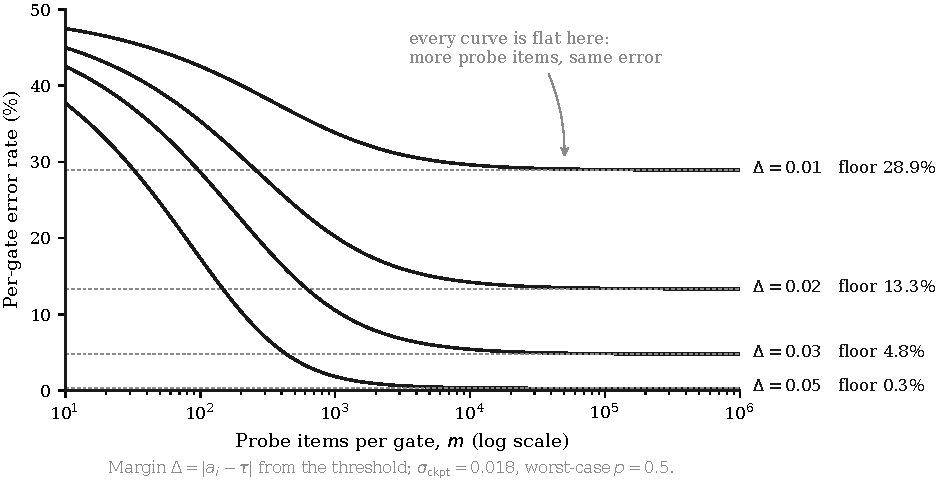
\includegraphics[width=\textwidth]{fig_reliability_floor.pdf}
\caption{Per-gate error rate against probe budget, for four distances from the
threshold. Each curve falls while sampling noise dominates and then stops,
because the checkpoint term in Equation~\ref{eq:var} does not shrink with $m$.
The dashed asymptote is the floor. No probe budget reaches below it, and the
cost of trying grows linearly along the horizontal axis. Generated by
\texttt{make\_figures.py} from the formula \texttt{gate\_reliability.py}
tabulates.}
\label{fig:floor}
\end{figure}

\subsection{Measuring the noise floor on curriculum probes}
\label{sec:measured}

The value $\sigma_{\text{ckpt}} = 0.018$ is borrowed from ARC-Challenge and from
seed variation at 1B scale, neither of which is a probe a curriculum would gate
on. We are not aware of a published test--retest reliability figure for a mastery
bit (fix a set of items, freeze the probe, score it at successive checkpoints,
and report how often the bit changes), so we measured one.

Our harness supports this without new training runs. The gate probe set is
constructed once per run and frozen, then re-scored at every evaluation, so the
same items are graded against successive parameter vectors and variation in the
measured accuracy contains \emph{no} resampling component. It is model-state
wobble, which is exactly the quantity Equation~\ref{eq:var} calls
$\sigma_{\text{ckpt}}$. Across 124 logged runs we take every skill that reached
$\tau$ at least once and track it from first clearance onward.

Separating the arms is essential. Where a scheduler keeps sampling every skill
for the whole run, a cleared skill is still being trained, so a bit that flips
cannot be decaying from withdrawal; the flip is instability. In gating and
staging arms the two causes are confounded. Table~\ref{tab:bitstability} reports
them apart.

\begin{table}[ht]
\centering
\small
\begin{tabular}{@{}lrrr@{}}
\toprule
& \multicolumn{2}{c}{Ours, $0.6$M synthetic} & Pythia-410m \\
\cmidrule(lr){2-3}\cmidrule(lr){4-4}
& Still sampled & Gated or staged & (always sampled) \\
\midrule
Nodes that ever cleared $\tau$ & 29 & 168 & 15 of 24 \\
Adjacent checkpoint pairs & 404 & 2{,}273 & 264 \\
$\sigma_{\text{ckpt}}$, median & $\mathbf{0.0228}$ & $0.0316$ & $\mathbf{0.0232}$ \\
$\sigma_{\text{ckpt}}$, interquartile range & $0.014$--$0.031$ & $0.018$--$0.073$ & $0.019$--$0.027$ \\
Pairs on which the mastery bit flipped & $5.7\%$ & $14.8\%$ & $\mathbf{11.4\%}$ \\
Nodes that later fell back below $\tau$ & $37.9\%$ & $58.3\%$ & $\mathbf{53.3\%}$ \\
\bottomrule
\end{tabular}
\caption{Test--retest reliability of the mastery bit, from
\texttt{mastery\_bit\_stability.py} and \texttt{openckpt\_analysis.py}. The left
two columns are our synthetic runs at $\tau = 0.9$. The right column is
Pythia-410m over its final twelve saved checkpoints (steps $132$k--$143$k) on a frozen 960-item SciQ
probe partitioned into 24 nodes, at $\tau = 0.60$. Pythia never withdraws
content, so every node there is under continuous training and no flip can be
decay from withdrawal. $\sigma_{\text{ckpt}}$ is computed from first differences,
removing drift so genuine learning is not counted as noise.}
\label{tab:bitstability}
\end{table}

The two settings differ by nearly three orders of magnitude in parameter count,
and use different data, vocabularies, thresholds and probe formats. They agree on $\sigma_{\text{ckpt}}$ to within two percent,
$0.0228$ against $0.0232$. We did not expect agreement that close and do not
claim the agreement is meaningful beyond the obvious reading, which is that both
measurements put the quantity in the same place and both put it \emph{above} the
$0.018$ we assumed. Table~\ref{tab:reliability} therefore understates the floor;
at the measured value the error at a $0.02$ margin rises from $13.3\%$ to
$19.0\%$. We keep $0.018$ as the conservative choice.

The mastery bit flips on $11.4\%$ of adjacent checkpoint pairs, so a gate
consulted at step $t$ and again one checkpoint later disagrees with itself
roughly one time in nine. And $53.3\%$ of nodes that once cleared the threshold
later fell back below it, on a model that never stopped training on anything.
Both figures are worse on the real run than on ours.

\begin{observation}[Aggregate stability conceals gate churn]
\label{obs:conceal}
Across the twelve checkpoints, overall probe accuracy moves within a band of
$0.012$ (standard deviation $0.0035$). Between steps $139$k and $140$k it
\emph{rises}, from $0.571$ to $0.577$, while the number of nodes above threshold
\emph{falls} from 13 to 9. A scheduler watching aggregate loss would see steady
progress at exactly the moment a third of its certified nodes revoked
themselves.
\end{observation}

\begin{figure}[ht]
\centering
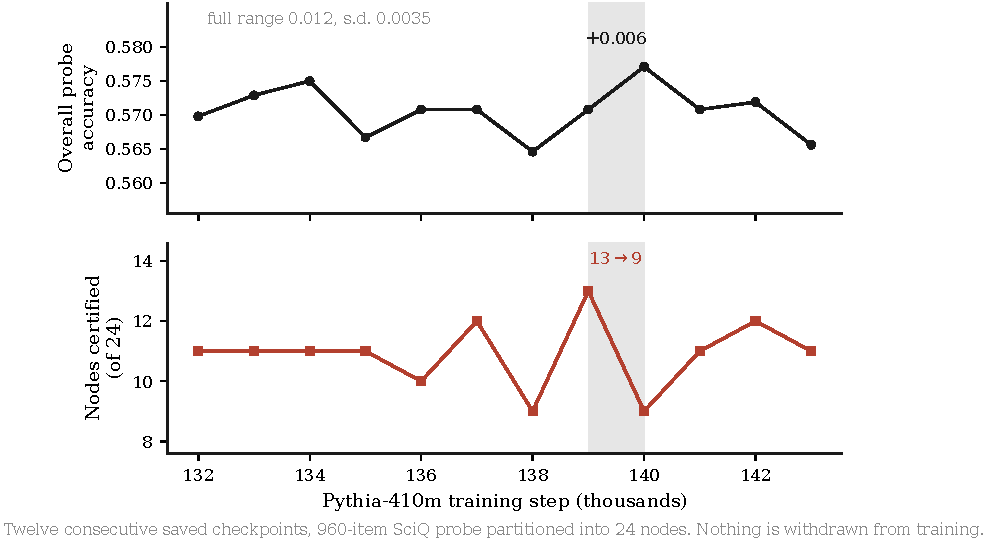
\includegraphics[width=\textwidth]{fig_pythia_churn.pdf}
\caption{The quantity a gate reads does not hold still, and the quantity a
scheduler usually watches gives no warning. Aggregate accuracy on the frozen
probe (top) stays inside a $0.012$ band for the whole window, while the number
of nodes clearing $\tau = 0.60$ (bottom) swings between 9 and 13. Shaded is the
adjacent pair of Observation~\ref{obs:conceal}, where accuracy rises by $0.006$
and four certified nodes revoke themselves at the same time. Generated from the
sweep output \texttt{openckpt\_\allowbreak results.csv} by
\texttt{make\_\allowbreak figures.py}.}
\label{fig:churn}
\end{figure}

Observation~\ref{obs:conceal}, plotted in Figure~\ref{fig:churn}, rules out the
natural dismissal that the flips merely track a model getting worse. They do not. The model is improving on the
same probe set while the gates churn beneath it. What moves is the position of
individual nodes relative to a threshold, which is the only thing a gate can
see. Aggregate competence holds steady.

\paragraph{Limits of this measurement.} Our synthetic estimate rests on 29
skill-runs at $0.6$M parameters. The Pythia measurement is larger in scale but
narrower in extent. It covers twelve checkpoints, one model size, one probe, and
nodes that are equal-size partitions of SciQ rather than semantically coherent
skills. A
curriculum node would be a coherent topic, and coherence might either stabilise a
node or make it more brittle; we cannot say which from this design. Neither
measurement establishes the value at frontier scale. What they jointly establish
is that $\sigma_{\text{ckpt}}$ is comfortably positive on probes of the kind a
gate would read, in both a toy setting and a real pretraining run, which is what
Proposition~\ref{prop:floor} requires.

\subsection{How much the floor depends on that value}

\paragraph{Sensitivity.} If the true value were a quarter of the published low
end, the floor at a $0.02$ margin would fall from $13.3\%$ to essentially zero.
The sensitivity is real and we report it. At $\sigma_{\text{ckpt}} \in \{0.005,
0.010, 0.018, 0.0228\}$ the floor at a $0.02$ margin is $0.00\%$, $2.28\%$,
$13.33\%$, $19.02\%$. What the argument requires, however, is only that
$\sigma_{\text{ckpt}} > 0$, meaning some checkpoint-to-checkpoint variation
exists that no probe budget removes. Every published measurement, and the one we
made ourselves, puts it well above zero, and Section~\ref{sec:decay} gives the
mechanism.

\paragraph{The Gaussian form.} Accuracy estimates are bounded in $[0,1]$ and the
sampling component is binomial, so the normal tail in
Proposition~\ref{prop:floor} is an approximation. It is a good one near the
thresholds gates actually use, and more importantly the conclusion does not
depend on it. For \emph{any} noise distribution with positive scale that does not
shrink with $m$, the misclassification probability converges to a positive
constant. The Gaussian only fixes the numbers in
Table~\ref{tab:reliability}, not the existence of the floor.

\subsection{Three further error sources, all in the same direction}

\paragraph{Multiple testing.} A gate is a threshold test repeated across nodes
and checkpoints. With $M_0$ genuinely unmastered nodes at per-gate error
$\alpha$, expected false unlocks are $M_0\alpha$ by linearity of expectation, and
holding family-wise error to $\alpha$ requires testing each gate at $\alpha/M_0$
\citep{dunn1961multiple}. Family-wise control is the punishing target; a
curriculum can more plausibly tolerate a fixed \emph{fraction} of bad unlocks, in
which case false-discovery control applies and is far less costly at large $M_0$
\citep{benjamini1995controlling}. Either way the correction tightens as the
curriculum grows.

Repeated looks compound the problem independently. At nominal $\alpha = 0.05$,
cumulative type-I error reaches $19.3\%$ after 10 sequential tests and $37.4\%$
after 100, and under the null the median number of tests before a spurious
rejection is 613 \citep{armitage1969repeated}.\footnote{The 613 figure is
verbatim from Armitage et al. The inflation percentages are read from their
normal-case table via two independent secondary sources, cross-checked against
the exponential-case table we retrieved directly, with which they agree to three
decimals. Note also that their correlation structure comes from an accumulating
sample, whereas a gate re-scores a fixed probe set against a changing model; the
true inflation for our setting lies somewhere between their curve and the
independent-looks curve, which reaches $40.1\%$ at 10 looks.} A node re-probed
often enough unlocks eventually whether or not it was ever learned.

\paragraph{Adaptive reuse.} Gating branches the training schedule on repeated
queries to a held-out set, which is adaptive data analysis.
\citet{dwork2015preserving} show naive empirical means on a shared holdout
support only $O(n)$ adaptive queries, and that the failure ``requires only a
single round of adaptivity.'' Their synthetic demonstration is the cleanest
illustration available. With $n = 10{,}000$ holdout points and \emph{uniformly
random labels}, so that no classifier can exceed $50\%$ true accuracy, naive
reuse reports over $63\%$ \citep{dwork2015reusable}. \citet{steinke2015interactive}
show no computationally efficient mechanism supports more than ${\approx}n^2$
adaptive queries. For $M \cdot K = 10^6$ gate decisions at tolerance $0.05$, the
efficient-mechanism bound of \citet{dwork2015preserving} requires a probe set of
order $10^7$ items, times an unspecified constant.

\paragraph{Calibration in the best case.} The most mature deployed gating systems
supply the empirical floor. Bayesian knowledge tracing
\citep{corbett1995knowledge} underpins the Cognitive Tutor, where mastery is by
convention declared at a posterior of $0.95$ \citep{fancsali2013optimal}.
Simulating that gate with run-time parameters \emph{matched to the generating
process}, the most favourable case available, \citet{fancsali2013optimal}
still find under $5\%$ premature unlocks and
over-practice for roughly $30\%$ of learners. They describe the threshold as ``a
tunable parameter that controls the relative frequency of the two types of
mastery assessment errors,'' which is to say that any gate has an irreducible
error rate in both directions and the threshold only chooses the exchange rate
between them. That is a decades-refined
instrument under ideal conditions. A pretraining gate has no calibration data,
runs orders of magnitude more decisions, and faces the adaptive rather than the
cooperative case.

\section{The Cost and Accuracy of the Graph}
\label{sec:graphcost}

\subsection{Construction is quadratic and has never been done at scale}

Establishing a prerequisite relation requires a judgment per ordered pair.
Sorting-based reductions to $O(n \log n)$ do not apply, because they presume a
total order and prerequisite structure is a partial order that annotators cannot
keep transitively consistent. The revealing data point is that the authors of the
leading LLM concept-graph paper declined to run all pairs on a \textbf{322-node}
graph ($103{,}362$ ordered pairs), citing API cost, and fell back to edge
sampling \citep{yang2024cgprompt}.

A pretraining corpus is not 322 nodes. Dolma reports $4.37 \times 10^9$ documents
at 3T tokens \citep{soldaini2024dolma}, and RedPajama-v2's deduplicated partition
reports $2.08 \times 10^{10}$ documents at 30.4T tokens \citep{weber2024redpajama}.
Taking $10^{10}$ nodes and the verified per-judgment cost of \$0.003
\citep{gilardi2023chatgpt}, a single unreplicated pass over $n^2/2 = 5 \times
10^{19}$ pairs costs on the order of $10^{16}$ dollars. Even at $10^4$ nodes, a
curriculum four orders of magnitude coarser than the corpus, the bill is about
\$300{,}000 for one judgment per pair, before replication or human adjudication
at MTurk's roughly \$0.09 per annotation.

For structure learned rather than annotated, the cost is worse in kind.
Skill-it's brute-force graph estimator is $O(Hk^2)$ \emph{training runs}
\citep{chen2023skillit}. The structure is discovered by training, so to know the
graph you must first run the experiment the graph was meant to save. In education
the same economics appear as authoring labor of 200--300 hours per hour of
instruction \citep{aleven2010rule} for knowledge bases of a few hundred items,
reduced to 50--100 by tooling.

\subsection{Accuracy is capped below what gating requires}

The binding constraint is annotator reliability rather than algorithmic
capability. When \citet{liang2017recovering} scored their
own thirteen annotators against their own majority-vote consensus, individual
annotators achieved F1 $0.75 \pm 0.08$ at Fleiss' $\kappa = 0.42$. That is a
self-consistency ceiling. Anything scoring above it is fitting annotator noise.
\citet{alzetta2023annotation} find unscaffolded protocols fall to Cohen's $\kappa$
between $0.01$ and $0.31$, and, directly relevant to scaling, agreement
\emph{falls} as the concept set grows, from $0.62$ at 132 concepts to $0.25$ at
353, with a 14-point F1 penalty on models trained from the noisier labels.

Automatic extraction performs about as one would expect against that ceiling. It
scores F1 $0.63$--$0.75$ in-domain but ${\approx}60\%$ accuracy on balanced
cross-domain data \citep{liang2015measuring}, $0.761$ on LectureBank \citep{li2019lecturebank},
and $0.777$ for GPT-4 zero-shot, which collapses to $0.416$ under a
chain-of-thought prompt, so a presentational change moves the edge set by 35 F1
points \citep{yang2024cgprompt}. Two facts make even these optimistic. All are
measured on artificially balanced test sets while the true base rate of
prerequisite relations is $2.15\%$ \citep{li2019lecturebank}; carrying the best
operating point to natural prevalence gives precision ${\approx}0.10$ and F1
${\approx}0.17$.\footnote{Our arithmetic, not a reported figure. LectureBank's
best classifier scores precision $0.832$ at recall $0.703$ on a balanced set,
implying a false-positive rate of $0.703\,(1/0.832 - 1) = 0.142$. At the reported
prevalence of $921/42{,}750 = 2.15\%$, precision becomes $(0.0215 \times 0.703) /
(0.0215 \times 0.703 + 0.9785 \times 0.142) = 0.098$, and F1 $= 0.17$. This
assumes the classifier's true-positive and false-positive rates are
prevalence-invariant, which is the standard assumption when transporting an
operating point.} And the highest reported scores come from datasets expanded by
transitive closure, which leaks logically implied pairs across the
cross-validation split.

\subsection{The graph is often degenerate even when correctly learned}

\citet{chen2023skillit} report that on two of three real datasets their learned
skill graph collapsed to an extremum their own definition excludes, at $97.4\%$
dense on Alpaca and $3.9\%$ dense on Pile of Law. The dense one bought $0.007$
validation loss over random sampling. One pays quadratic cost to discover whether
the graph contains usable information at all.

\section{What a Wrong Graph Costs}
\label{sec:wrong}

The literature on curriculum \emph{ordering} largely finds that order barely
matters, and that reversed orderings often match forward ones.
\citet{wettig2024qurating} report $+0.6$ in-context-learning points for a
forward difficulty curriculum and $+0.5$ for its reverse. This is sometimes read
as reassurance that a wrong graph is harmless. That reading conflates gating with
ordering. A soft curriculum reweights a pool that remains fully available, while
a gate \emph{withholds} content until a threshold clears. A wrong edge in a soft
curriculum delays; a wrong edge in a gated curriculum blocks.

We are not aware of a prior measurement of this distinction for a gated
curriculum, and a systematic review of the prerequisite-graph literature
conducted for this paper likewise found none. Our runs happen to supply the
$2 \times 3$ design that separates the two. Every cell in
Table~\ref{tab:wrongdag} is the same configuration (reference-chain task,
$L{=}5$, $6{,}000$ steps, $\tau = 0.9$, replay fraction $0.5$), varying only
which prerequisite order is supplied and whether the scheduler advances when a
probe clears or when a clock expires.

\begin{table}[ht]
\centering
\small
\begin{tabular}{@{}lrrr@{}}
\toprule
Graph supplied & Clock advancement & Gated advancement & Gate effect \\
\midrule
Correct (natural) & $\mathbf{0.835 \pm 0.102}$ & $0.792 \pm 0.108$ & $-0.043$ \\
Scrambled & $0.324 \pm 0.127$ & $0.129 \pm 0.098$ & $\mathbf{-0.195}$ \\
Reversed & $0.103 \pm 0.000$ & $0.098 \pm 0.007$ & $-0.005$ \\
\midrule
None (\texttt{shuffle}) & \multicolumn{2}{c}{$0.491 \pm 0.036$} & n/a \\
\bottomrule
\end{tabular}
\caption{Final accuracy, mean $\pm$ standard deviation, from
\texttt{paper\_infeasibility/ordering\_vs\_gating.py}. $n = 5$ for the correct
graph and the shuffled reference, $n = 3$ for the degraded graphs. The rightmost
column is what probe gating adds relative to a clock marching through the
identical order.}
\label{tab:wrongdag}
\end{table}

\begin{figure}[ht]
\centering
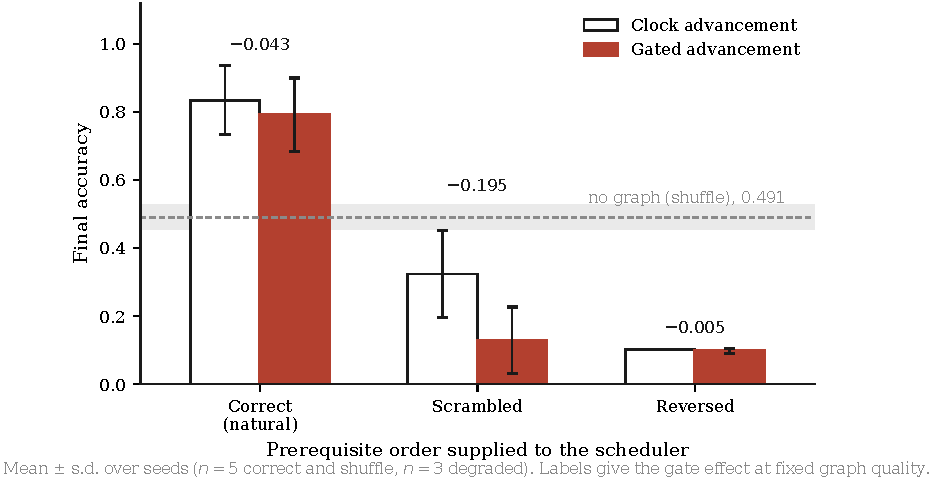
\includegraphics[width=\textwidth]{fig_ordering_vs_gating.pdf}
\caption{The same six cells as Table~\ref{tab:wrongdag}. Comparing across groups
prices the prerequisite \emph{ordering}, which is worth $+0.344$ against no graph
when correct and $-0.388$ when reversed. Comparing within a group prices the
\emph{gate}, holding the supplied order fixed, and that comparison is negative in
all three. Generated by \texttt{make\_figures.py} from
\texttt{ordering\_vs\_gating.py}.}
\label{fig:wrongdag}
\end{figure}

Reading the table by rows prices the \emph{structure}; reading it by columns
prices the \emph{gate}, and the two come apart. Figure~\ref{fig:wrongdag} shows
both readings at once.

\begin{observation}[The ordering carries the benefit, and the payoff is asymmetric]
\label{obs:asym}
Against no graph at all, clock-staged training through a correct order is worth
$+0.344$, through a scrambled order $-0.167$, and through a reversed order
$-0.388$. Prerequisite structure genuinely helps when correct, and the downside
of getting it wrong exceeds the upside of getting it right.
\end{observation}

\begin{observation}[The gate never pays, at any level of graph correctness]
\label{obs:wrong}
Holding the supplied graph fixed and switching only the advancement rule, probe
gating scores $-0.043$ against a clock on a correct graph, $-0.195$ on a
scrambled graph, and $-0.005$ on a reversed graph. The sign is negative in three
of three conditions.
\end{observation}

The strength of evidence differs across those three cells and we will not
overstate it. Only the scrambled gap exceeds two standard errors of the
difference ($2.10$ SE), and it does so at $n = 3$; the correct-graph gap is well
within noise at $0.65$ SE, and the reversed cells are both at the floor. What is
consistent is the direction. Across three independent degradations of the graph,
gating is never the better rule. The gap is widest exactly where one would
expect it, on a partially wrong graph, where a clock moves on while a gate waits
at a stage whose prerequisite will never clear.

The mechanism is visible in the unlock logs. Under the reversed graph the gate
produced \emph{zero} unlocks across all three seeds, and under the scrambled
graph it managed one unlock in one seed of three; the correct-graph runs unlocked
three to four of five stages. The gate did not impose a worse ordering; it
stopped the curriculum from advancing at all. Relaxing the threshold from $0.90$ to $0.80$
changes nothing ($0.129$ either way), because the blocked stage is at chance,
not near the threshold.

This is where Section~\ref{sec:graphcost} bites. Structure is worth $+0.344$ when
correct, but a realistically extracted graph carries roughly one true edge for
every nine asserted ones at natural base rates, and the gate subtracts from
whatever remains. The nearest published analogue is Q-matrix misspecification in
psychometrics, where flipping a single bit per item produces high
misclassification and, notably, more data does not repair it
\citep{rupp2008qmatrix}.

One feature of this comparison works against us. Our
\texttt{shuffle} arm never stops sampling mastered skills, so it is a wasteful
policy and a weak comparator. That makes Observation~\ref{obs:asym}
\emph{conservative} in the direction that matters. A stronger graph-free baseline
would raise the $0.491$ reference, shrinking the measured value of correct
structure and widening the measured damage of wrong structure. It does not affect
Observation~\ref{obs:wrong} at all, since that comparison never touches
\texttt{shuffle}.

Our result is also not isolated. BabyAI's own curriculum experiment found that
pretraining on \texttt{GoToObjMaze} made the \texttt{GoTo} target level
\emph{worse} (444--602k versus 341--409k demonstrations from scratch), concluding
that ``current deep learning methods often can not take the full advantage of
available curriculums'' \citep{chevalierboisvert2019babyai}. OpenAI Five ablated
its one hand-designed structural scaffold and found it ``may not have been
necessary in the end'' \citep{berner2019dota}.

\section{Pre-commitment Is Dominated by Reading the Model's State}
\label{sec:static}

A clarification is needed before the evidence, because this section can look like
it contradicts the last one. Section~\ref{sec:wrong} found that a \emph{static}
clock schedule through a correct order beats undifferentiated shuffling by
$+0.344$; that is static structure winning, and we are not retracting it. The
claim here is narrower and compatible. \emph{Given} some structure worth
exploiting, a scheduler that reads the model's current state beats one that
pre-commits to a fixed allocation. Section~\ref{sec:wrong} compares structure
against no structure. This section compares two ways of using the same structure.

We should also be plain that our experiments do not test this. We ran no online
arm, so everything in this section rests on the literature. What our runs
contribute is the adjacent result that among pre-committed rules gating is
worse than a clock, which is consistent with the ordering below but does not
establish it.

The sharpest evidence that adaptivity rather than structure does the work comes
from inside the leading pro-graph paper. \citet{chen2023skillit} build a skill
graph and then use it two ways. Statically, they allocate sampling weight by
graph structure and hold it fixed; online, they use the \emph{same} graph but
reweight each round by current per-skill validation loss. The online variant
wins by $9.9$ to $25.9$ accuracy points at the halfway mark. Because the graph is
identical in both arms, this isolates adaptivity from structure. Their own
diagnosis is precisely the staleness argument, that a static allocation ``will
continue to allocate the same weight to that skill throughout training'' after it
has been learned.

The cost comparison is equally lopsided. Adaptive Data Optimization reweights
online from per-domain scaling-law fits with no proxy model at under $0.4\%$
wall-clock overhead, and posts the best average downstream score at both 124M and
1.3B \citep{jiang2025ado}. DoReMi's static optimized weights cost $8\%$ of
main-model FLOPs \citep{xie2023doremi} and, at 1.3B, lose to weighting each domain
by its token count. ADO's own footnote closes the obvious escape hatch, noting
that ``a static mixture is nothing but a fixed stationary curriculum throughout
the training, [so] this computational difficulty applies to finding a static
mixture too.''

\citet{graves2017automated} observed that uniform sampling is ``a surprisingly
strong benchmark'' because
``learning is dominated by gradients from the tasks on which the network is
making fastest progress, inducing a kind of implicit curriculum.'' Gradient
descent already runs an approximate learning-progress scheduler for free, so a
prerequisite graph is competing against the curriculum SGD induces on its own. And \citet{portelas2019teacher} find an adaptive teacher beating a
hand-designed Oracle curriculum $80\%$ to $68\%$ ($p < 0.02$), with the
hand-designed schedule winning early and losing late, the signature of a
pre-commitment that cannot track the learner.

\begin{remark}[Nobody charges the gate]
\citet{narvekar2020curriculum} define the strong-transfer accounting we adopt
here and then observe that the field ``has usually treated curriculum generation
as a sunk cost.'' The pattern holds in the systems that spend the most on
certification. OpenAI's automatic domain randomization devotes half of all worker
iterations to evaluation and then recycles that data into training ``to avoid
wasting a large amount of data for only ADR'' \citep{akkaya2019solving}. XLand's
gate requires ten Monte Carlo episodes per policy per \emph{proposal} task, with
rejected proposals unaccounted \citep{openended2021xland}. ACCEL plots against
student gradient updates ``as opposed to total number of environment
interactions'' \citep{parkerholder2022accel}.

To our knowledge, no prior work isolates the marginal value of a prerequisite
graph against a strong graph-free adaptive baseline with certification charged.
We state this as a search result rather than a theorem. The literature
bifurcates. Graph-based methods \citep{svetlik2017automatic,narvekar2020curriculum} benchmark
a DAG against learning from scratch or against a hand-designed sequence, while
graph-free adaptive methods \citep{graves2017automated,matiisen2017tscl,%
portelas2019teacher,jiang2021plr} benchmark adaptivity against uniform sampling.
Nobody runs the two-by-two. The nearest comparison is ALP-GMM against its
hand-designed Oracle, which pits adaptivity against a hand-designed
\emph{sequence}, not a certified graph, with no cost charged to either arm. We
checked each of these specifically; a counterexample would not surprise us, and
we would rather hedge the claim than overstate it.
\end{remark}

\section{Why the Human Case Differs}
\label{sec:human}

Mastery learning works for humans, and the mechanism is what fails to transfer.

Humans have a hard capacity bottleneck, roughly four chunks in the focus of
attention \citep{cowan2001magical}, that applies \emph{only to novel
information}. As \citet{sweller2019cognitive} put it, all novel information is
first processed by a capacity- and duration-limited working memory, and ``once
information is stored in long-term memory, the capacity and duration limits of
working memory disappear.'' Task difficulty is therefore a joint property of the
material and the learner's long-term memory, since mastering a prerequisite
collapses many simultaneously-active elements into one retrievable chunk. Below capacity,
learning proceeds; above it, it does not happen at all. Mastery gating in humans
is a threshold-crossing intervention against a hard serial constraint, and the
expertise reversal effect \citep{kalyuga2003expertise} is its signature. Once the
schema is consolidated, the scaffolding becomes redundant load.

A transformer has no such bottleneck. Context length, parameter count, and FLOPs
per token are fixed by architecture and do not expand as a function of what has
already been learned. There is no chunking operation that frees per-step
capacity. Consequently the failure mode gating exists to prevent does not occur.
A human lacking prerequisites fails discontinuously, so ordering is a feasibility
constraint, whereas a model lacking prerequisites receives a smaller and noisier
gradient and updates anyway, so ordering is at most an optimization.

The human evidence is also weaker than its reputation.
The two-sigma figure rests on two Chicago dissertations, ${\approx}20$--$33$
students per cell in a single school over three weeks, in which the control group
never received the parallel retest forms the treatment groups took
\citep{anania1983influence,bloom1984twosigma}. \citet{vanlehn2011relative} puts
human tutoring at $d = 0.79$ and intelligent tutoring systems at $0.76$.
\citet{slavin1987mastery} finds a median effect of $+0.04$ on standardized tests,
a conclusion \citet{kulik1990effectiveness} concede for the studies using
standardized criterion tests.

The premise that securing prerequisites reduces downstream corrective load is
empirically false. \citet{arlin1984time} tracked time-to-mastery over four years
and found the slowest-to-fastest ratio \emph{grew} from $2.5{:}1$ in first grade
to $4.2{:}1$ by fourth. \citet{arlin1983time} found mastery students
learned twice as much but took twice as long, and on a four-day retention test
the control group retained more \emph{per hour of instruction}. Under a fixed
budget, that is a loss.\footnote{We take both Arlin results as reported in
\citet{slavin1987mastery}, which quotes the figures and the study designs; we did
not retrieve the primary papers. Anyone relying on these numbers should confirm
them at source, and Slavin cites two separate 1984 Arlin papers of which we could
verify only one.} Even within a well-tuned deployed system,
\citet{cen2007overpractice} found that $58\%$ of 4{,}102 practice opportunities
in the Cognitive Tutor were spent after mastery had already been reached, while
genuinely hard skills went under-practiced.

\section{Threats to Validity}
\label{sec:threats}

We state the strongest objections we know of, including two that apply to our own
evidence.

\paragraph{Our baselines are weak in one direction.} Our \texttt{shuffle} arm
never stops sampling mastered skills, so it is a wasteful policy by construction.
Any speedup measured against it overstates the value of the machinery being
tested, including our own graph-free tracker. Reported $\kgf$ values should be
read as upper bounds on graph-free value, not estimates.

\paragraph{Our experiments are small and synthetic.} All arms train ${\sim}0.6$M
parameter models on synthetic addition and reference-chain tasks, five orders of
magnitude below the regime the paper reasons about. It matters what job each
result is doing. The forgetting result exists to falsify an assumption (the
monotonicity premise of the exposure model), and a single clean counterexample
suffices for that, independent of scale. The wrong-graph result establishes that
gating and ordering are different interventions, which is a qualitative claim
about a mechanism. Neither is offered as a pretraining magnitude, and every
section that extrapolates is labelled a derivation.

\paragraph{Forgetting may shrink with scale, which cuts against us.}
\citet{tirumala2022memorization} find that the forgetting baseline rises
monotonically with model size, so larger models forget \emph{less}. Our $62.3\%$
figure therefore sits at the wrong end of a scale trend, and we should not be
read as predicting anything like it at 7B. We think the argument survives for two
reasons. First, as above, the result's function is to refute monotonicity, not to
size an effect, and \citet{chang2024acquire} independently measure decay inside
real OLMo pretraining with a fitted power law. Second, the direction of the trend
does not help a gate. Even the reduced forgetting that
\citet{tirumala2022memorization} measure is nonzero and asymptotic, so a retired
node still decays and still needs re-probing. A reader who rejects our magnitude
should still accept that the schedule cannot retire anything permanently.

\paragraph{Nobody would build a graph over $10^{10}$ documents.} Agreed, and the
$10^{16}$ figure in Section~\ref{sec:graphcost} is a scale marker rather than a
proposal anyone has made. The objection has a real form, though, which is that a
coarser graph is affordable. The difficulty is that coarsening trades one problem
for another. A graph over a few thousand topical nodes costs on the order of
$10^5$ dollars to judge once and, because its edges no longer correspond to
individual training items, it constrains the scheduler only through a mapping
from documents to nodes that must itself be built and maintained. The regime
where the graph is cheap is the regime where its edges are too coarse to gate on,
and the regime where edges are precise enough to gate on is the regime where
there are too many of them. We know of no analysis that escapes this, but we have
not proved that none exists.

\paragraph{The learning-rate objection.} \citet{luo2025lrdecay} argue that
curriculum null results may be artifacts of learning-rate schedules tuned for
uniform ordering, since a curriculum wants a much higher terminal learning rate
($\approx 10^{-3}$ versus $10^{-5}$). This is the most serious methodological
objection to the ordering literature we cite. We note that their own ceiling
after correcting it is $+1.64\%$, and that the correction requires abandoning
decay-to-zero, which is an additional unpriced cost.

\paragraph{Adaptive overfitting is empirically milder than theory predicts.}
\citet{recht2019imagenet} measure an $11$--$14\%$ ImageNet drop and then
explicitly conclude it is \emph{not} caused by adaptivity, and subsequent work
attributes most of the gap to replication bias and model similarity. Our
Section~\ref{sec:reliability} argument therefore rests on worst-case theory in a
regime where the observed human-driven case is benign. We think the distinction
holds (a gating controller branching on probe outputs at high frequency is a
deliberate optimizer against the probe signal, which is the adversarial analyst
the theory models, and the query count is orders of magnitude larger than any
Kaggle competition), but a reader who rejects that distinction should treat
Proposition~\ref{prop:floor}, which does not depend on adaptivity at all, as the
load-bearing result.

\paragraph{Curricula do sometimes help.} \citet{zucchet2025facts} demonstrate a
genuine positive curriculum result in self-supervised pretraining, calling it ``a
rare example in which data curricula benefit (self-)supervised learning.'' Their
intervention is a \emph{distributional warm-up}, adjusting item frequencies over
time, not mastery gating. We regard the distinction as central. The literature
supports distribution scheduling and undercuts gating, and conflating them is the
easiest way to dismiss the argument in either direction.

\paragraph{Falsifiers.} Our position would be falsified by any of the following.
A $\sigma_{\text{ckpt}}$ near zero measured at pretraining scale on gate-style
probes, which would remove the reliability floor. Our own measurement in
Section~\ref{sec:measured} gives $0.023$, but on small synthetic tasks. A gated
arm beating a clock arm advanced through the \emph{same} prerequisite order, at
any graph quality, which is the comparison Section~\ref{sec:wrong} runs and which
went against the gate in three of three conditions. A gated arm beating a
graph-free adaptive arm under matched budget with certification charged. A
prerequisite extractor exceeding $0.75$ F1 against a gold standard not built from
the same annotator pool. Or a demonstration that a wrong edge under gating
degrades gracefully rather than blocking advancement outright.

\section{Conclusion}

The case against mastery-gated pretraining does not need the idealized exposure
model, and is stronger without it. Mastered skills decay, so gates must recur;
recurring certification costs between $8\%$ and $125\%$ of a training budget at
realistic curriculum scale; and no probe budget makes those gates reliable,
because the quantity being thresholded moves by more between adjacent checkpoints
than the decision needs to resolve. Meanwhile the graph that the gates release is
quadratic to build and degenerate on two of three real datasets where it has been
learned honestly. Its accuracy is capped near $0.75$ F1 by human
self-consistency, and near $0.10$ precision at natural base rates.

The cleanest way to see the problem is to separate the two things a gated
curriculum does. Section~\ref{sec:wrong} varies the prerequisite order and the
advancement rule independently, and they dissociate. Staging through a correct
order is worth $+0.344$ against no graph at all, while replacing the clock with a
probe gate is negative on a correct graph, on a scrambled one, and on a reversed
one. Whatever a curriculum is worth, it is the ordering that earns it. The gate
is the part that costs money to run, cannot be resolved reliably at any probe
budget, and subtracts from the result. The alternative is therefore online
machinery that reads the model's current state at under half a percent overhead,
on top of the implicit curriculum that gradient descent already runs for free.

Section~\ref{sec:measured} contributes the number the argument most needed and
that we could not find in the literature, a test--retest reliability figure for a
mastery bit, measured twice. On our synthetic runs the bit flips on $5.7\%$ of
adjacent checkpoint pairs; on Pythia-410m's final twelve checkpoints it flips on
$11.4\%$, with $53.3\%$ of nodes that once cleared the threshold later falling
back below it while the model trains continuously on everything. The two settings
differ by three orders of magnitude in scale and agree on $\sigma_{\text{ckpt}}$
to within two percent, and both exceed the value we assumed.

The finding we would put in front of anyone considering this design is
Observation~\ref{obs:conceal}. Between two adjacent Pythia checkpoints, aggregate
probe accuracy rose while the number of nodes above threshold fell from 13 to 9.
Nothing was withdrawn and nothing got worse. The quantity a gate thresholds
simply does not hold still, and it does not hold still for reasons that buying
more probe items cannot touch.

\bibliographystyle{plainnat}
\bibliography{infeasibility}

\end{document}
